\section{Array}
Array adalah variabel jamak, yang mempunyai banyak elemen yang diacu dengan satu nama yang sama. Array (atau larik dalam bahasa indonesia) bukanlah tipe data dasar seperti integer atau boolen, Array adalah sebuah tipe data bentukan yang terdiri dari kumpulan tipe data lainnya. Menggunakan array akan memudahkan dalam membuat kelompok data, serta menghemat penulisan dan penggunaan variabel. berikut sebagai contoh
 \begin{lstlisting}
<?php
    $a = array("budi", 20, 58.5);
?>
\end{lstlisting}
Array dalam PHP juga merupakan tipe data, bukan sekedar variabel. Berikut merupakan jenis array dalam PHP:
\subsection{Array Berindeks}
Array berindeks adalah array yang diindeks berdasarkan nomor/angka. Indeks array pada umumnya dimulai dari angka 0. Anda bebas mendefinisikan indeks dengan nilai yang Anda tentukan.

\begin{table}[h]
\caption(Array Berindeks}
\centering
\begin{tabular}
\hline
\textbf{10}&\textbf{20}&\textbf{30}&\textbf{40}&\textbf{50}\\
\hline

\begin{lstlisting}
 $a[0]
\end{lstlisting}  & 

\begin{lstlisting}
 $a[1]
\end{lstlisting} &

\begin{lstlisting}
 $a[2]
\end{lstlisting} &

\begin{lstlisting}
 $a[3]
\end{lstlisting} &

\begin{lstlisting}
 $a[4]
\end{lstlisting}\\
\hline
\end{tabular}
\label{tabel : Array Berindeks}
\end{table}


Contoh diatas menunjukan array dengan 5 buah elemen. Elemen pertama ($a[0]) bernilai 10, elemen
kedua ($a[1]) bernilai 20, dan seterusnya. Dalam array berindeks, antara kunci (indeks) dan nilai tidak
memiliki keterkaitan.

\subsection{Array Asosiatif}
Array asosiatif adalah array yang diindeks berdasarkan nama tertentu. Letak perbedaan antara array berindeks dan array asosiatif adalah hanya terletak pada penamaan indeksnya saja.
\begin{table}[h]
\caption(Array Asosiatif}
\centering
\begin{tabular}{|c|c|c|c|c|}
\hline
\textbf{10}&\textbf{20}&\textbf{30}&\textbf{40}&\textbf{50}\\
\hline

\begin{lstlisting}
 $a["satu"]
\end{lstlisting}  & 

\begin{lstlisting}
 $a["dua"]
\end{lstlisting} &

\begin{lstlisting}
 $a["tiga"]
\end{lstlisting} &

\begin{lstlisting}
 $a["empat"]
\end{lstlisting} &

\begin{lstlisting}
 $a["lima"]
\end{lstlisting}\\
\hline
\end{tabular}
\label{tabel : Array Asosiatif}
\end{table}

Array diindeks berdasarkan nama, bukan berdasarkan nomor. Pada contoh diatas indeks array bertipe string. Pada umumnya array asosiatif digunakan untuk merepresentasikan sesuatu yang kunci dan nilainya memiliki keterkaitan, misalnya sebagai berikut.

\begin{lstlisting}
 <?php
  $kota = array("jkt" => "jakarta", "bdg" => "bandung", "sby" => "surabaya");
 ?>
\end{lstlisting}  


\section{Membuat Array}
Array dapat dibuat melalui dua cara, yaitu dengan menggunakan fungsi array() atau dengan membuat elemen-elemen array dan mengisikan nilai-nilai ke dalam elemen-elemen tersebut secara langsung.
Berikut ini contoh pembuatan array dengan menggunakan fungsi array().

\item{Untuk Array Berindeks}
\begin{lstlisting}
<?php
 $matakuliah = array ("pemograman web", "database", "keamanan jaringan",
 "sistem informasi", "rekayasa perangkat lunak");
 ?>
\end{lstlisting}

\item{Untuk Array Asosiatif}
\begin{lstlisting}
<?php
$detailmk = array ("kode" => "TKB5218", "nama" => "pemograman web 2", "sks" => 2);
?>
\end{lstlisting}

Berikut ini contoh pembuatan array dengan cara langsung membuat variabel array dan mengisikan nilai ke dalamnya.

\item{Untuk array berindeks}
\begin{lstlisting}
<?php 
$matakuliah[0] = "pemograman web"; 
$matakuliah[1] = "database"; 
$matakuliah[2] = "keamanan jaringan"; 
$matakuliah[3] = "sistem informasi"; 
$matakuliah[4] = "rekayasa perangkat lunak"; 
?>
\end{lstlisting}

\item{Untuk array asosiatif}
\begin{lstlisting}
<?php 
$detailmk["kode"] = "TKB5218"; 
$detailmk["nama"] = "pemograman web 2"; 
$detailmk["sks"] = 2; 
?>
\end{lstlisting}

\subsection{Mengakses Elemen Array}
Setelah array dibuat, langkah selanjutnya adalah mengakses nilai-nilai yang terkandung di dalamnya.
Cara mengakses elemen array sangatlah sederhana. Karena elemen array berupa nilai, maka kita dapat
memperlakukannya seperti layaknya variabel.
Kita dapat menempatkan nilai yang diakses ke dalam suatu variabel atau dapat juga diproses secara
langsung baik dalam perhitungan maupun ditampilkan langsung.
Berikut ini adalah contoh mengakses nilai array ke dalam suatu variabel.
\lstinputlisting[firstline=1, lastline=9]{src/array.php}

Berikut ini adalah contoh mengakses elemen array secara langsung
\lstinputlisting[firstline=1, lastline=23]{src/akses_array.php}

\subsection{Fungsi-fungsi yang berhubungan dengan array}
Berikut ini beberapa fungsi yang dapat digunakan pada variabel bertipe array.
\begin{figure}[!htbp]
 \centering
 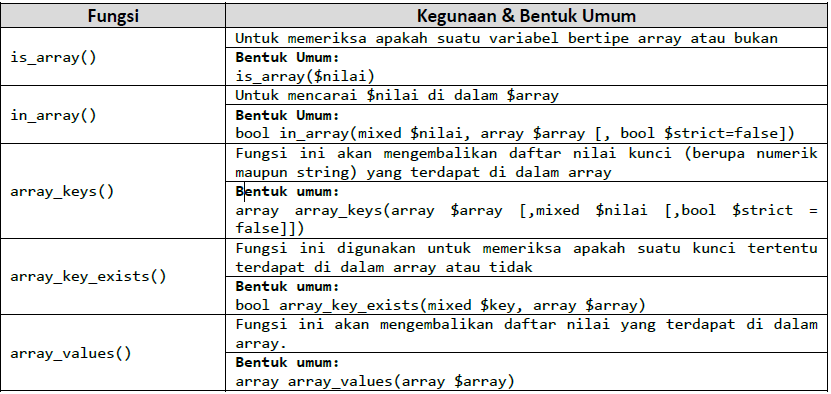
\includegraphics[width=.90\textwidth]{figures/fungsi_array.png}
\end{figure}

\begin{figure}[!htbp]
 \centering
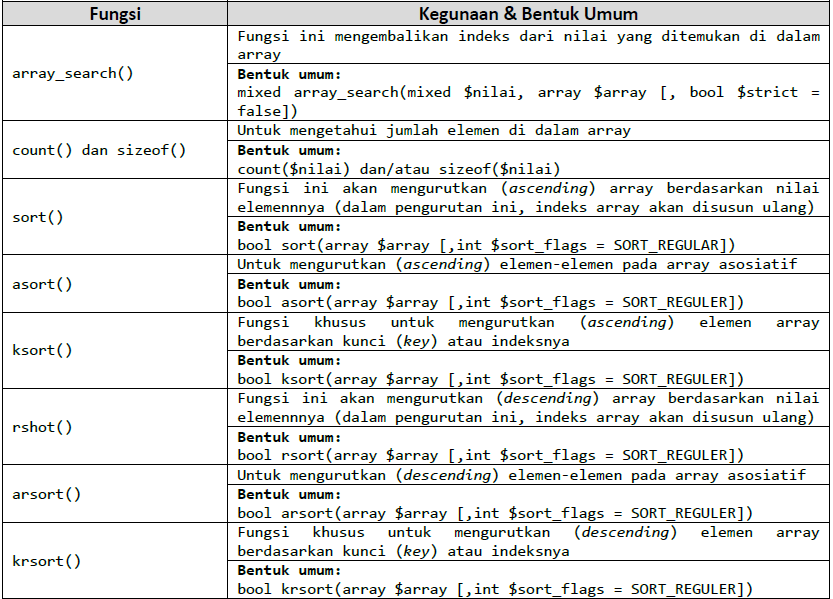
\includegraphics[width=.90\textwidth]{figures/fungsi_array2.png}
 \caption{Fungsi-fungsi yang berhubungan dengan array}\label{fig:inputchapter}
\end{figure}

